% Used Template for Computer Science Tripos Part II project dissertation, by Martin Richards, Simon Moore
\documentclass[12pt,a4paper,twoside,openright]{report}
\usepackage[pdfborder={0 0 0}]{hyperref}    % turns references into hyperlinks
\usepackage[margin=25mm]{geometry}  % adjusts page layout
\usepackage{graphicx}  % allows inclusion of PDF, PNG and JPG images
\usepackage{verbatim}
\usepackage{docmute}   % only needed to allow inclusion of proposal.tex
\usepackage{amsfonts}
\usepackage{amsmath}
\usepackage{tikz}
\usepackage{float}
\usepackage{todonotes}
\usepackage{cleveref}
\usepackage{booktabs}
\usepackage{mathtools}


\edef\restoreparindent{\parindent=\the\parindent\relax}
\usepackage{parskip}
\restoreparindent

\renewcommand{\vec}[1]{\mathbf{#1}}
\DeclareMathOperator*{\argmax}{argmax}
\DeclareMathOperator*{\argmin}{argmin}

\crefformat{section}{\S#2#1#3} % see manual of cleveref, section 8.2.1
\crefformat{subsection}{\S#2#1#3}
\crefformat{subsubsection}{\S#2#1#3}

\crefformat{figure}{Figure~#2#1#3}

\newcommand{\R}{\mathbb{R}}

\raggedbottom                           % try to avoid widows and orphans
\sloppy
\clubpenalty1000%
\widowpenalty1000%

\renewcommand{\baselinestretch}{1.1}    % adjust line spacing to make
                                        % more readable

\begin{document}
\pagenumbering{gobble}

\bibliographystyle{unsrt}

%%%%%%%%%%%%%%%%%%%%%%%%%%%%%%%%%%%%%%%%%%%%%%%%%%%%%%%%%%%%%%%%%%%%%%%%
% Title


\thispagestyle{empty}
\rightline{\Large\textbf{Ian Tai}}
\vspace*{50mm}
\begin{center}
\rule{\linewidth}{1pt}\vspace{5mm}
\LARGE\textbf{Learning the Stock Market: Deep Learning and Sentiment
Analysis-Based Stock Price Prediction}
\rule{\linewidth}{1pt} \\[10mm]
\Large\textsc{Computer Science Tripos -- Part II \\[5mm]
Trinity College \\[5mm]
\today}  % today's date
\end{center}

%%%%%%%%%%%%%%%%%%%%%%%%%%%%%%%%%%%%%%%%%%%%%%%%%%%%%%%%%%%%%%%%%%%%%%%%%%%%%%
% Proforma, table of contents and list of figures
\pagestyle{plain}
\setcounter{page}{1} 
\chapter*{Proforma}
\pagenumbering{roman}
{\large
\begin{tabular}{ll}
Name:               & \bf Ian Tai                      \\[-2pt]
College:            & \bf Trinity College                     \\[-2pt]
Project Title:      & \bf Learning the Stock Market: Deep Learning \\[-2pt]
& \bf and Sentiment Analysis-Based Stock Price\\[-2pt]
& \bf Prediction \\[-3pt]
Examination:        & \bf Computer Science Tripos Part II, May 2018  \\[-2pt]
Word Count:         & \footnotemark \\[-3pt]
Project Originator: & \bf Ian Tai                    \\[-2pt]
Supervisors:         & \bf Dr Sean Holden                    \\[-2pt]
& \bf Prof Stephen Satchell
\end{tabular}
}
\footnotetext[1]{This word count was computed
by \TeX count}

\stepcounter{footnote}


\section*{Original Aims of the Project}

Deep Learning has increasingly been applied to many fields of industry. Among Finance,
the applications of Deep Learning in predicting stock market prices is an increasingly
popular research field. This dissertation proposes a method of stock price prediction
using a combination of Long Short-Term Memory Recurrent Neural Networks and a variety
of Sentiment Analysis techniques. The project aims to apply this method to collected 
news headlines from selected news agencies on Twitter and stock price data from the 
latter two quarters of 2017.

\section*{Work Completed}

This project has been successful; all success criteria have been met. I collected, parsed, and converted
financial data from a Bloomberg Terminal. I 
built a data collection and processing system for the Twitter dataset. I implemented
Gaussian and Multinomial Naive Bayes Classifiers, and used the
Scikit-Learn library for implementing Multi-Class Support Vector Machines and
Semi-Supervised Support Vector Machines for sentiment analysis. Finally, I built
a Long Short-Term Memory Recursive Neural Network for stock price prediction. The techniques
proposed for predicting stock market prices have developed results that match, if not exceed,
state-of-the-art accuracies, and can benefit financial and machine learning research in this field.

\section*{Special Difficulties}

Finding appropriate Twitter datasets proved to be more difficult than was foreseen, which led to
trying various sources of data, different models of classification, and ultimately, manual classification
of the data for train/test purposes.
 
\newpage
\section*{Declaration}

I, Ian Tai of Trinity College, being a candidate for Part II of the Computer
Science Tripos, hereby declare
that this dissertation and the work described in it are my own work,
unaided except as may be specified below, and that the dissertation
does not contain material that has already been used to any substantial
extent for a comparable purpose.

\bigskip
\leftline{Signed: Ian Tai}

\medskip
\leftline{Date: \today}

\tableofcontents

{\listoffigures \let\cleardoublepage\clearpage \listoftables}

\newpage
\section*{Acknowledgements}

I would like to thank the following people for the help they have given me:

\todo[inline]{TODO: COMPLETE AFTERWARDS}

%%%%%%%%%%%%%%%%%%%%%%%%%%%%%%%%%%%%%%%%%%%%%%%%%%%%%%%%%%%%%%%%%%%%%%%
% now for the chapters

\pagestyle{headings}

\chapter{Introduction}

\pagenumbering{arabic}

This dissertation describes experimentation with several
techniques for stock price prediction, and proposes a novel method for tackling this problem.
The focus of the project is to combine machine learning-based sentiment analysis with deep learning-based 
stock price prediction. For this purpose, I implemented several sentiment analysis classifiers,
used different feature extraction techniques, and built a state of the art deep Long Short-Term Memory Network. 
These components combine into the proposed stock price prediction system.

\todo[inline]{TODO: talk about how successful the project was}

\section{Motivation \& Aims}

Machine learning is perhaps the most famous topic in Computer Science in the current decade.
Being the focus of much media attention, and one of the most researched areas for the largest
technology companies, it is in the somewhat unique position of having captivated both the
public and the experts in the field. The underlying reasons for this are unsurprising --
the ability for computers to perform at superhuman levels for tasks that were previously
considered human specialities is bound to catch attention.

Perhaps even more interesting is the ability for machine learning (more specifically
deep learning) to perform
admirably on tasks that were previously thought exceedingly difficult,
even for humans. These tasks, such as near-instantaneous language translation\cite{Sutskever14}, and
accurate medical diagnosis of difficult patients\cite{Litjens17, Lee17}, show not only the prospect of machine learning
replacing human jobs, but also its application to new fields that were previously
unaccessible. Stock price prediction is one of these new areas.

Stock price prediction presents a formidable machine learning problem on several levels.
The signal to noise ratio inherent to any stock price dataset renders the task difficult
for many traditional learning models. Moreover, it is debated whether stock prices are
even predictable -- under the Efficient Market Hypothesis, an efficient capital market fully reflects
all relevant information in determining security prices \cite{Malkiel89}. Since all past prices and
information are available to the market, correct predictions, if possible, should immediately be
taken advantage of, and the resulting market adjustment quickly nullifies any possible advantage.
It logically follows that an efficient market is arguably unpredictable, and behaves in the manner of a Random Walk.

However, several factors contribute to potential inefficiency in practical markets --
there usually exists some latency in market information availability and absorption, varying liquidity levels
of different commodities and equities, different levels of information availability, and countless other
real-life factors. Thus, it is argued that there exists a window for prediction\cite{Buffett10, Chan03, Basu77}.

The rise of deep learning techniques has allowed models to learn complicated and highly-nonlinear 
patterns. Most relevant to this project is the advent of Recurrent Neural Networks (RNNs) in learning tasks, from
Google Duplex's most recent automated phone calls\footnote{\url{https://blog.google/products/assistant/io18/}}
powered by Deepmind's Wavenet\cite{Oord16}, to optical character recognition\cite{Breuel13}, to
robotic surgery control\cite{Mayer08}, to time-series prediction\cite{Malhotra15, Lipton15}, and many more.
The inherent ability of RNNs to handle time-series data and learn long and short term dependencies makes
this architecture a prime candidate for stock price prediction.

The use of Twitter as a source of spreading news and information has also seen increasing importance in the past years,
most notably shown by how President Donald Trump regularly releases important news regarding the United States 
on his Twitter page. Tweets\footnote{Tweets are the name given to Twitter posts} from News Agencies are often
a good source of quick information, as the most relevant headlines are often posted. This essentially creates
a filter for good content that we are able to use for sentiment analysis.

I will be using sentiment analysis of Tweets from financial news agencies and technical analysis of stock
price data to feed into a Deep Long Short-Term Memory Network to predict stock prices.
By applying machine learning techniques in a novel approach to this learning problem,
I will be contributing a new perspective on the optimal ways of finding the solution
that is so desired in the Finance industry. Moreover, the unique noisy nature of this
dataset makes it an inherently difficult machine learning problem, and one that is inherently
difficult even for humans.

\section{Challenges}
\label{sec:introChallenges}

The challenges posed by the inherent noisy nature of stock price data renders this problem
high risk -- there is a fair chance that approaches may not even succeed. Moreover, the
sentiment analysis problem also poses risk -- I must be able to either find a relevant labelled dataset,
or gather my own and manually label it. Unfortunately, such a dataset was unable to be found.

Manual labelling restricts the possible approaches that
can be taken, since the dataset will not be large enough for a deep learning approach. This topic
is discussed in detail in \cref{sec:prepRej} and \cref{sec:impFailed}.
Because of the need for sentiment and financial data with matching time periods, the limitation of manual labelling
also restricts the number of stocks and financial markets that can be explored in this project. Therefore there
is also risk in selecting an appropriate financial dataset.

The financial dataset was collected using a Bloomberg Terminal. This is a program that is ubiquitous
in the finance industry, for collecting stock or commodity prices, statistical analysis, viewing breaking news,
gathering historical data, and much more. Collecting data required that I learn how to use the software --
though this should be trivial for a Computer Science student, the number of features and abundance of
financial lingo makes this task significantly harder than was expected.

Choosing the correct machine learning and deep learning models can also be difficult. Since
there are an abundance of machine learning models, and it is critical that I understand the theories and
properties of each in order to gauge their suitability for this task.

\section{Related Work}

The papers introducing Long Short-Term Memory Networks and Deep Long Short-Term
Memory Networks are discussed below.

There are few publications regarding the combination of sentiment analysis with financial data to predict stock
prices, though there is literature on each approach to the stock price prediction problem.
It is also important to note that papers on each topic may be untrustworthy or dubious, due to the nature of
the learning problem and its financial appeal. There are also few papers that attempt to predict intra-day
prices, rather than end-of-day, due to the larger amount of noise inherent to intra-day data.

\subsection{Recurrent Neural Networks}

The paper by Hochreiter et al. from 1997 introduced Long Short-Term Memory (LSTM) Networks
as a solution to the vanishing/exploding gradient problem in normal Recurrent Neural Networks (RNNs)\cite{Hochreiter97}.
This was a breakthrough that allowed RNNs to be used in practical applications, such as time series
prediction. The LSTM was revised by Gers et al. in 1999, introducing the forget gate, which tackled
the problem of catastrophic failure in the case of long serial inputs\cite{Gers99}.
In 2013, Graves et al. introduced Deep LSTM Networks, which was the concept of
stacking LSTM in hidden layers, similar to the architecture of regular Deep Neural Networks. This provided
an extraordinary boost to the learning abilities of the network, as deep networks are able to learn much
more complex and highly non-linear patterns\cite{Graves13}.

\subsection{Sentiment Analysis for Price Prediction}

The first paper relating sentiment and stock prices is by Wuthrich et al. in 1998\cite{Wuthrich1998}. The study
was conducted on whether negative sentiment in the news would affect the various stock market indices around the world,
sampled on a daily interval.
The study used a carefully curated collection of relevant phrases, such as `dollar falter' and `technology
rebound strongly'. The number of overall occurrences of these phrases was counted, and the result was used
in a system that generates `probabilistic rules'.

A paper published by Tetlock et al. in 2008\cite{Tetlock08} studied whether negative sentiment in the news would affect 
a company's earnings as well as its stock price on a daily interval. In this case, sentiment was measured as the frequency 
of negative words in a news article, according to the Harvard-IV-4 
dictionary\footnote{\url{http://www.wjh.harvard.edu/~inquirer/homecat.htm}}.
The method for modelling was linear regression, a standard method in economics. This was one of the first studies to try
to actually predict stock prices, rather than a simple rise or fall prediction.

The first paper to use Twitter as its data source is by Bollen and Huina from 2010\cite{Bollen11}.
The study used OpinionFinder\footnote{\url{http://mpqa.cs.pitt.edu/opinionfinder/}} and Google's Profile of Mood States
for feature extraction, which simply outputs whether a Tweet is `Calm, Alert, Sure, Vital, Kind, [or] Happy'. 
This is fed into a Self-Organizing Fuzzy Neural Network and a Granger causality analysis calculation\footnote{A statistical test for determining
whether one time series forecasts another} to
predict stock prices on a daily interval.

\subsection{Financial Data for Price Prediction}

There are a large number of papers that focus on predicting stock prices using technical indicators of
financial data using deep learning. Most of these are based on data sampled on a daily interval.
The first instance was in 1988 by White, who used a Multilayer Perceptron (MLP) with one hidden layer.
However, the end result was a failure\cite{White98}.

A more recent paper by Bao et al. from 2017 uses LSTM Networks and Stacked Autoencoders\footnote{Stacked autoencoders are an unsupervised deep learning
algorithm for efficient encodings} (SAE)\cite{Bao17}.
This study used Wavelet transforms to de-noise financial data, with SAEs being used to
generate high-level features from the de-noised data. These features were then fed into a deep LSTM network. This method
was used to predict the prices of several stock market indices on a daily interval.

\subsection{Sentiment Analysis Combined with Financial Data}

One of the few papers that presents the combination of sentiment analysis and financial data to predict stock
prices is by Zhao et al.\cite{Zhai07}. The paper presents a Support Vector Machine model that uses Bag of Words
and technical financial indicators to predict the rise or fall of a single stock on a daily interval.

\chapter{Preparation}
\label{sec:prep}

This chapter includes all of the work that was completed before implementation began.
This includes the theory behind each Machine Learning model (\cref{sec:introNN},
\cref{sec:introSVM}, and \cref{sec:introNB}), 
an outline of the project's requirements (\cref{sec:introReq}), tools and libraries
considered and used (\cref{sec:introTool}), the starting point
for my project (\cref{sec:introStart}), and the development model and
early outline for implementation (\cref{sec:introImpl}).

\section{Neural Networks}
\label{sec:introNN}

The theory regarding Recursive Neural Networks and
Long Short-Term Memory Networks in this section is partially adapted from \cite{Goodfellow-et-al-2016,
Hochreiter97, Gers99, Graves13}.

\subsection{Introduction}

Before delving into Recurrent Neural Networks (RNNs), we must first discuss
the basics of Machine Learning (ML). An ML algorithm is one that learns from
data. Mitchell (1997) provides a definition for learning:
``A computer program is said to learn from experience E with respect to some
class of tasks T and performance measure P, if its performance at tasks in T, as
measured by P, improves with experience E."\cite{Mitchell97} 

The use of a recurrent neural network in my project is in the manner of
supervised learning. Supervised learning is a subset of ML,
where all given data is labelled, such that each input, a vector of \textbf{features} (distinguishing
numerical characteristics of the input) $\vec{x} \in \R^m$,
is associated with a label $y$. This label can either be a discrete variable where 
$y \in C = [C_1, C_2, C_3, ..., C_n]$,
in the case of classification, or a continuous variable where $y \in \R$, in the case of regression.
The use of RNNs in this project is limited to regression.

A supervised learning algorithm for regression, given a training sequence
\begin{equation}
\vec{s} = ((\vec{x_1}, y_1), (\vec{x_2}, y_2), (\vec{x_3}, y_3), ... , (\vec{x_n}, y_n))
\end{equation}

where $(\vec{x_1}, y_1)$ is a training input, learns a function $h: \R^m \rightarrow \R$,
a hypothesis, that approximates a match between an input feature vector $\vec{x}$ to a
result $y$.

After learning this hypothesis function, the algorithm can then be used to predict test
samples $\vec{x'}$. We can then run accuracy measurements and goodness-of-fit tests on
the resulting outputs, given we know the original labels $y'$.

\subsection{Artificial Neurons}
\label{sec:prepNeurons}

A neural network is a network of artificial neurons that each takes an input $\vec{x}$,
and runs a linear combination of the input feature vector $\vec{x}$, weights $\vec{w}$, and a bias $b$,
fed through an activation function $\sigma$. The formulation is detailed below:

\begin{equation}
y = \sigma (\vec{wx} + b)
\end{equation}

The activation function is used to ensure the output stays within a preset bound,
usually either $[0,1]$ or $[-1,1]$. Typical activation functions are as follows:
\begin{align}
\intertext{Logistic Function (Sigmoid):}
&\sigma(x) = \frac{1}{1+e^{-x}}\\
\intertext{Rectified Linear Unit (RELU):}
&\sigma(x) = \text{max}(0,x)\\[10pt]
\intertext{Hyperbolic Tangent (tanh):}
&\sigma(x) = \frac{e^x - e^{-x}}{e^x + e^{-x}}
\end{align}\\*

\begin{figure}[h]
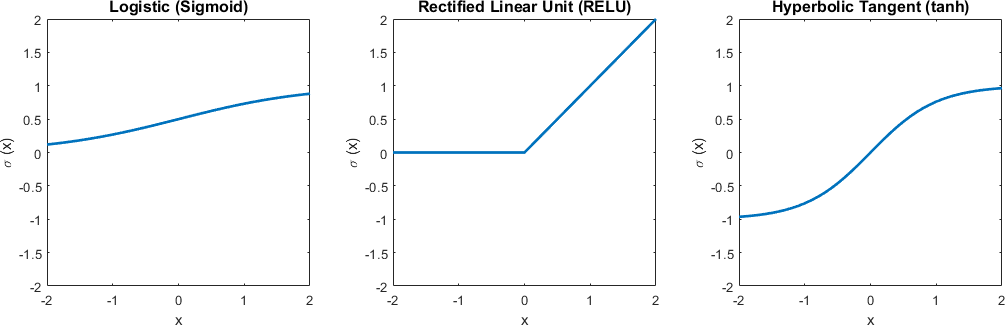
\includegraphics[width=\textwidth]{ActivationFunsCrop.png}
\caption{Plots of sigmoid, RELU, and hyperbolic tangent functions}
\end{figure}

The output is then fed as either an input to other artificial neurons, or is the overall
output of the neural network.

\subsection{Training}
\label{sec:introTraining}

The training of the network using the training set first includes initialization of the 
weights and biases. Initialization will be covered in depth in the Implementation section
for the Long Short-Term Memory RNN (\cref{sec:ImplLSTM}).

For a basic NN, such as the Multi-Layer Perceptron (MLP), the output of the NN is
observed by simple \textbf{feed-forward propagation}. This means in the directed graph
of the NN architecture, calculated values for each training example ($\vec{x_i}$)
flow from neuron to neuron across layers, and the eventual
output is run through a final activation function to obtain the final result.

This output ($y_i'$) can then be fed into the \textbf{loss function} to calculate the error for this
training example. A typical loss function for this purpose is the Sum of Squared Errors 
function\footnote{Adapted from Dr Sean Holden's Machine Learning and Bayesian Inference Part II course \cite{Holden18}}:

\begin{equation}
\text{E}(\vec{x}, \vec{y}, \vec{w}, \vec{b})  = \sum_{i=1}^{n} (y_i - y_i')^2
\end{equation}

where $\vec{w}$ and $\vec{b}$ specify the weights and biases of the NN respectively, 
$\vec{x}$ is the set of training examples,
$\vec{y}$ is the set of training labels, n is the number of training examples, and $y_i$ and $y_i'$
are the training label and output value for training example $i$, respectively.

Based on the output of the loss function, the NN can then adjust its weights and biases to minimize
loss. This adjustment is performed using \textbf{gradient descent}. This optimization algorithm
iteratively updates these parameters using the gradients calculated from the loss function until
convergence is reached. Different variations of gradient descent used for the Long Short-Term Memory 
network (LSTM) will be discussed further in the Implementation section for LSTMs
(\cref{sec:ImplLSTM}).

The gradients are calculated as follows:
\begin{align}
\vec{w_{t+1}} &= \vec{w_t} - \lambda \frac{\delta E(\vec{x}, \vec{y}, \vec{w}, \vec{b})}{\delta \vec{w}} \Big|_\vec{w_t}\\
\vec{b_{t+1}} &= \vec{b_t} - \lambda \frac{\delta E(\vec{x}, \vec{y}, \vec{w}, \vec{b})}{\delta \vec{b}} \Big|_\vec{b_t}
\end{align}
where $\vec{w_{t+1}}$ and $\vec{b_{t+1}}$ are the weight and bias vectors at iteration $t$, respectively.
The parameter $\lambda$ is known as the learning rate, a hyperparameter\footnote{Hyperparameters are configurable
settings for a Neural Network that are often manually tuned for optimal performance and desired run-time} for NNs.
The learning rate must be chosen carefully; if it is too small, the NN may take an exceedingly long time to reach
convergence during the training period, and if too large, the NN may never find an appropriate minimum.

\begin{figure}[H]
\centering
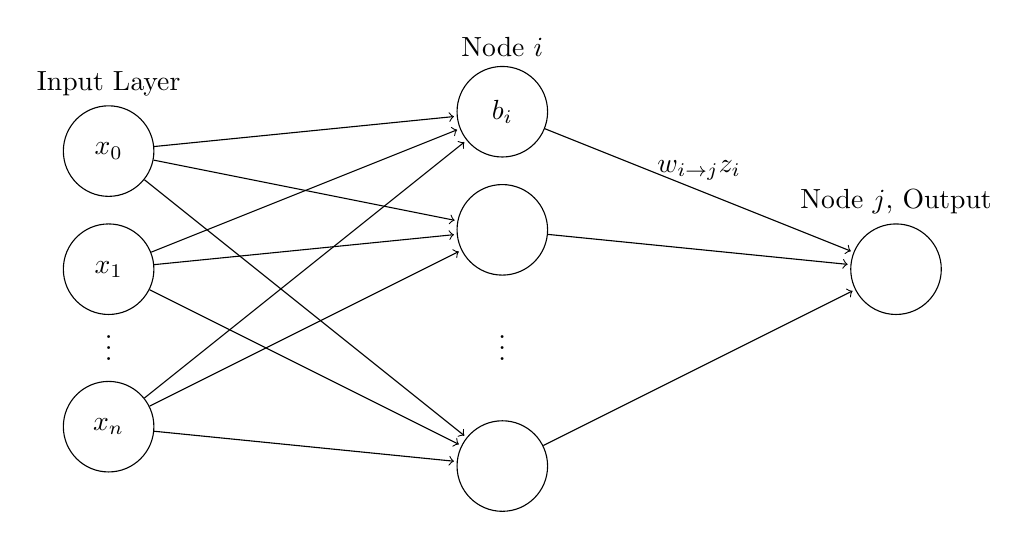
\begin{tikzpicture}[shorten >=1pt]
	\tikzstyle{unit}=[draw,shape=circle,minimum size=1.15cm]

	\node[label={Input Layer},unit](x0) at (0,3.5){$x_0$};
	\node[unit](x1) at (0,2){$x_1$};
	\node at (0,1.1){\vdots};
	\node[unit](xd) at (0,0){$x_n$};

	\node[label={Node $i$}, unit](h10) at (5,4){$b_i$};
	\node[unit](h11) at (5,2.5){};
	\node at (5,1.1){\vdots};
	\node[unit](h1m) at (5,-0.5){};

	\node[label={Node $j$, Output},unit](y2) at (10,2){};

	\draw[->] (x0) -- (h10);
	\draw[->] (x0) -- (h11);
	\draw[->] (x0) -- (h1m);
	
	\draw[->] (x1) -- (h10);
	\draw[->] (x1) -- (h11);
	\draw[->] (x1) -- (h1m);

	\draw[->] (xd) -- (h10);
	\draw[->] (xd) -- (h11);
	\draw[->] (xd) -- (h1m);

	\draw[->] (h10) -- (y2) node[midway, above] {$w_{i \rightarrow j} z_i$};

	\draw[->] (h11) -- (y2);

	\draw[->] (h1m) -- (y2);

\end{tikzpicture}
\caption[Layout of an MLP]{Layout of a Multi-Layer Perceptron\footnotemark}
\label{fig:MLP}
\end{figure}

\footnotetext{$w_{i \rightarrow j} z_i$ is the weight associated with the output
of node $i$ as the input to node $j$ multiplied by the output of node $i$, $z_i$. $b_i$ is the bias associated with node $i$.
Adapted from Dr Sean Holden's Artificial Intelligence I Part IB course \cite{Holden18AI1}}

The weights and biases at various levels of the NN are updated using \textbf{backpropagation}. Backpropagation
is the method used for calculating $\frac{\delta E(\vec{x}, \vec{y}, \vec{w}, \vec{b})}{\delta \vec{w}}$ and
$\frac{\delta E(\vec{x}, \vec{y}, \vec{w}, \vec{b})}{\delta \vec{b}}$ for every weight $w_{i \rightarrow j}$ and bias
$b_{i}$, as shown in \cref{fig:MLP}. This can be calculated directly, since the gradient at each node in a layer is
independent when the chain rule is applied, using the calculated gradients of any nodes that take the input from
node $j$. Thus, we apply backpropagation to find the gradient of each weight, starting from the output node and
working our way backwards until we reach the input feature vectors. This can be summarized into the following:

\begin{align}
\frac{\delta E(\vec{x}, \vec{y}, \vec{w}, \vec{b})}{\delta w_{i \rightarrow j}} &= z_i \sigma_j(a_j) \sum_k \delta_k w_{j \rightarrow k}\\
\intertext{\indent where}
a_j &= \sum_k w_{k \rightarrow j} z_k
\end{align}

where $k$ is any node that takes the output of node $j$, $z_i$ is the value output of node $i$,
$\sigma_j$ is the activation function for the node $j$,
and $\delta_k$ is the gradient for $w_{k \rightarrow j}$ that has already been calculated.
This formulation for calculating the weights' gradients can include the gradients for the bias, if we simply
label the bias as an extra weight, multiplied by an arbitrary $z = 1$. 

\subsection{Recurrent Neural Networks}
\label{sec:introRNN}

\begin{figure}[H]
\centering
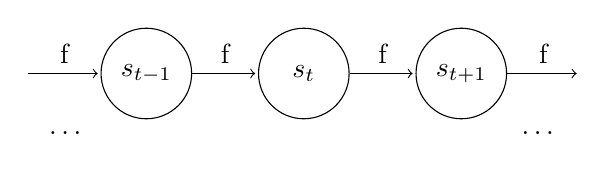
\begin{tikzpicture}[shorten >=1pt]
	\tikzstyle{unit}=[draw,shape=circle,minimum size=1.15cm]
	
	
	\node at (5,2.75){\dots};
	
	\node[unit](h0) at (6,3.5){$s_{t-1}$};
	\node[unit](h1) at (8,3.5){$s_{t}$};
	\node[unit](h2) at (10,3.5){$s_{t+1}$};
	
	\node at (11,2.75){\dots};
	
	\draw[->] (4.5,3.5) -- (h0) node[midway, above] {f};
	\draw[->] (h0) -- (h1) node[midway, above] {f};
	\draw[->] (h1) -- (h2) node[midway, above] {f};
	\draw[->] (h2) -- (11.5,3.5) node[midway, above] {f};
	
\end{tikzpicture}
\caption[States of a dynamic system]{The evolution of state in a system\footnotemark}
\label{fig:seqIn}
\end{figure}

Feed-forward networks require that each training example be input into the network in full, and that
each example be independent of each other. If we have the case of sequentially dependent inputs,
such as the state of a dynamic system that evolves with regards to a time $t$ (\cref{fig:seqIn}), then we can use
a Recurrent Neural Network.

\footnotetext{Each node represents the state at
some time $t$, which is mapped according to some underlying function f, to the state at time $t+1$}

\begin{figure}[H]
\centering
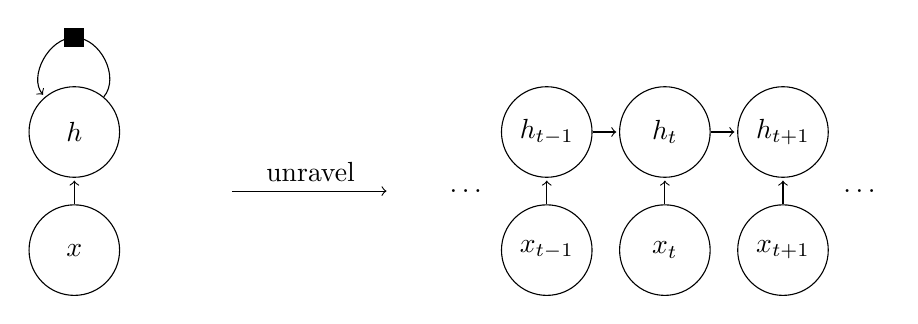
\begin{tikzpicture}[shorten >=1pt]
	\tikzstyle{unit}=[draw,shape=circle,minimum size=1.15cm]
	
	
	
	\node[unit](x) at (0,2){$x$};
	\node[unit](h) at (0,3.5){$h$};
	\draw[->] (x) -- (h);
	\draw[->] (h) to[out=50, in=0] (0,4.7) to[out=180, in=130] (h);
	\fill[black] (-0.125, 4.575) rectangle (0.125,4.825);
	
	\draw[->] (2,2.75) -- (4,2.75) node[midway, above] {unravel};
	
	\node at (5,2.75){\dots};
	
	\node[unit](h0) at (6,3.5){$h_{t-1}$};
	\node[unit](x0) at (6, 2){$x_{t-1}$};
	\draw[->] (x0) -- (h0);
	
	\node[unit](h1) at (7.5,3.5){$h_{t}$};
	\node[unit](x1) at (7.5, 2){$x_{t}$};
	\draw[->] (x1) -- (h1);

	\node[unit](h2) at (9,3.5){$h_{t+1}$};
	\node[unit](x2) at (9, 2){$x_{t+1}$};
	
	\node at (10,2.75){\dots};
	
	\draw[->] (x2) -- (h2);
	\draw[->] (h0) -- (h1);
	\draw[->] (h1) -- (h2);
	
\end{tikzpicture}
\caption[A simple RNN, in both its cyclic and unraveled form]{A simple RNN, in both its cyclic and unraveled form\footnotemark}
\label{fig:RNN}
\end{figure}

\footnotetext{(Left) The cyclic representation of an RNN. The rectangle in the cyclic arrow represents a delay of 1 time step.
(Right) The unraveled acyclic representation of the same RNN. This RNN processes information from a system at some time $t$ along
with the input passed from the network at time $t-1$, and uses this as an input for the network at time $t+1$}

In a feed-forward NN, there are no cycles in the network and all values simply propagate
towards the output node. A Recurrent Neural Network (RNN) introduces the concept of cycles, such
that the output of a node at time $t$ may be used as an input to a node at time $t+1$. \cref{fig:RNN}
shows an example of a simple RNN. From the cyclic graph on the left, we can simply unravel the graph
to have an acyclic computational graph.

There are several different design pattern for RNNs, each for a different use case:
\begin{itemize}
	\item
	RNNs that produce an output at each time step and have recurrent connections between hidden units
	at different time steps\footnote{Interestingly, such an RNN of a finite size can compute any function computable 
	by a Turing Machine\cite{Goodfellow-et-al-2016}}
	
	\item
	RNNs that produce an output at each time step and have recurrent connections only from an output
	at a previous time step to hidden units at the next time step
	
	\item
	RNNs that take a whole sequence of inputs before producing a single output
\end{itemize}

For the purposes of stock price prediction, the first design pattern is most useful. This is because
we expect our RNN to extract useful information about the state of the stock market and hold this
information within its hidden units, and this information may not be fully conveyed if we simply 
take the relevant output.

The relevant equations regarding the hidden state and output of an RNN are as follows:

\begin{align}
\vec{h}^{(t)} &= \tanh(\vec{b}_h + \vec{W}_hh\vec{h}^{(t-1)} + \vec{W}_xh\vec{x}^{(t)})\\
\vec{o}^{(t)} &= \vec{b}_o + \vec{W}_oh\vec{h}^{(t)}
\end{align}

where $\vec{h}^{(t)}$ represents the hidden state of the RNN unit at time $t$,
and $\vec{o}^{(t)}$ represents the output of the RNN unit at time $t$. The various
$\vec{W}$s represent represent the weights associated with the previous 
time step's hidden value, the current input, and the current hidden state value, respectively.
The variables $\vec{b}$ represent the biases of the hidden state and the
output, respectively\footnote{For reference, the weights are matrices, thus presented in upper case}.

A similar backpropagation algorithm to what was described in \cref{sec:introTraining} can be used
to train such an RNN -- however, we must also be backpropagating through the time steps. This algorithm
is called \textbf{backpropagation through time} (BPTT). This is simply the application of the
previous backpropagation algorithm to the unraveled computation graph of the RNN.

The key problem with the RNN that prevents it from being used in its purest form is the
\textbf{vanishing/exploding gradient problem}. The vanishing/exploding gradient problem
is the tendency for gradients that are propagated through many stages
to either vanish (become negligible) or explode (become disproportionately large). While the
former is only a problem with trying to model long-term dependencies, the latter can completely
disrupt the parameter optimization algorithm. The problem of the vanishing gradient follows naturally,
even without any unstably small gradients -- the weights given to long-term dependencies are
exponentially smaller than those given to short-term dependencies due to the repeated application
of the weight of the hidden unit over many time steps.

\subsection{Long Short-Term Memory Networks}
\label{sec:introLSTM}

The LSTM is perhaps the most popular solution to the vanishing/exploding
gradient problem of vanilla RNNs\footnote{Other solutions, such as the Gated Recurrent Unit (GRU), are
not within the scope of this project and will not be discussed}. The LSTM, a gated RNN, is based on the
idea of creating paths for dependencies through time where the derivatives will neither vanish
nor explode, by introducing variability to the connection weights between time steps and a learned
method of forgetting the old state.

The original proposal by Hochreiter and Schmidhuber for the LSTM states that it solves the
vanishing/exploding gradient problem by ``an efficient, gradient-based algorithm for
an architecture enforcing constant (thus, neither exploding nor vanishing)
error flow through internal states of special units (provided the gradient
computation is truncated at certain architecture-specific points)"\cite{Hochreiter97}.
This algorithm was the inclusion of an internal recurrence in addition to the outer
occurrence of an RNN. This internal recurrence, the `state' in \cref{fig:LSTMCell}
is preserved in the cell across time.

This design was later improved upon by Gers, Schmidhuber and Cummins,
who observed that the ``LSTM fails to learn to correctly process certain
very long or continual time series that are not \textit{a priori} segmented into 
appropriate training subsequences with clearly defined beginnings and ends"\cite{Gers99}.
This is because the values of the LSTM cell state can grow without bound if the
input stream is continuous. Thus, their paper introduced the forget gate,
whose role is to learn to reset the LSTM cell's memory contents when
the information is not needed anymore. \cref{fig:LSTMCell} shows
the resulting computational graph for an LSTM cell with the addition of forget gates.

\begin{figure}[H]
\center\textbf{LSTM Cell}
\centering
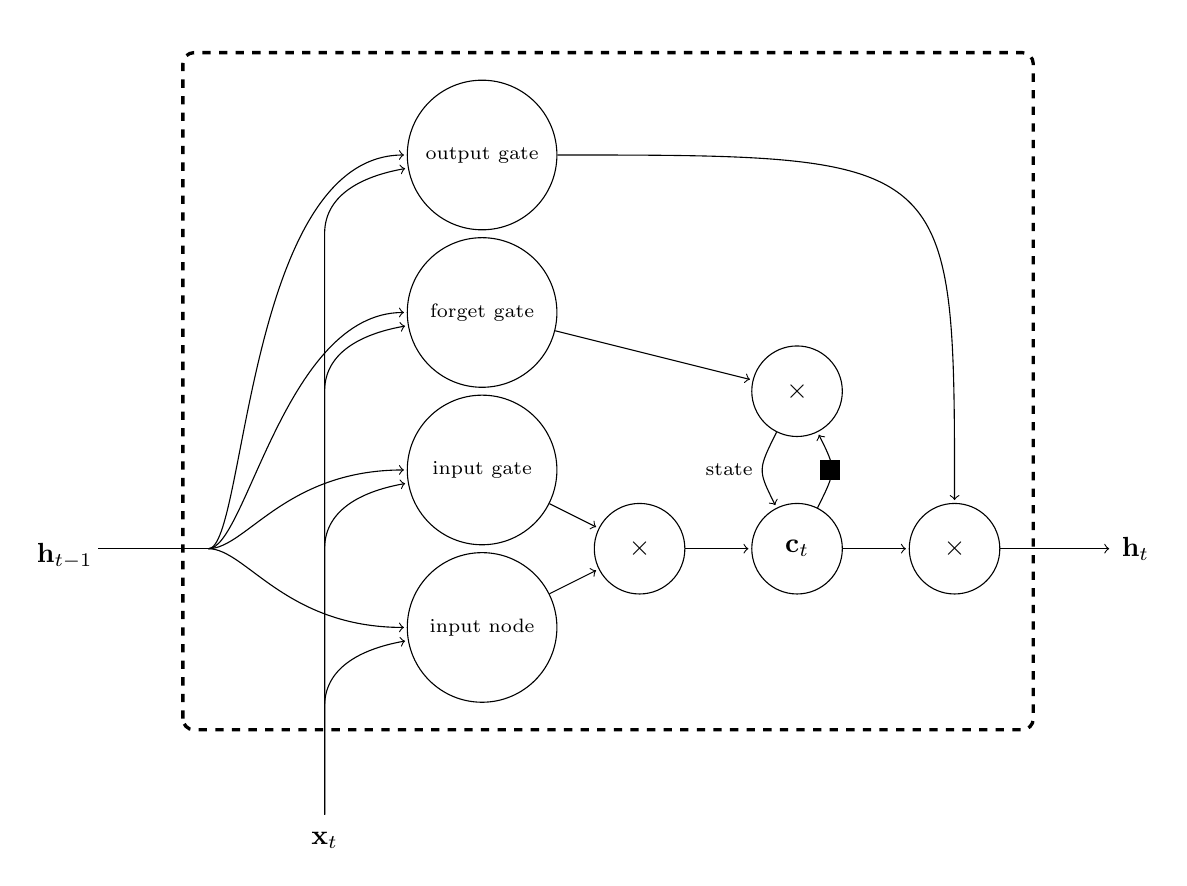
\begin{tikzpicture}[shorten >=1pt]
	\node(vspace) at (0,10){};
	
	\tikzstyle{unit}=[draw,shape=circle,minimum size=1.15cm]
	
	\tikzstyle{gate}=[draw,shape=circle,minimum size=1.9cm]
	
	\node(rec) at (1,0) {};
	\node at (1,-0.2){$\vec{x}_t$};
	\node[label={[align=center]$\vec{h}_{t-1}$}](recText) at (-2.3,3){};
	\node[minimum size=0.1pt,scale=0.1](in) at (0,3.5) {};
	\node(inHelp) at (-0.6,3.5) {};
	\node(trueIn) at (-2,3.5) {};
	
	\node[gate](input) at (3,2.5){\scriptsize{input node}};
	\node[gate](inGate) at (3,4.5){\scriptsize{input gate}};
	\node[gate](forget) at (3,6.5){\scriptsize{forget gate}};
	\node[gate](outGate) at (3,8.5){\scriptsize{output gate}};
	
	
	\node[unit](inx) at (5,3.5){$\times$};
	\node[unit](hiddenP) at (7,3.5){$\vec{c}_t$};
	
	\node[unit](hidden) at (7,5.5){$\times$};
	\node[unit](outx) at (9,3.5){$\times$};
	
	
	%\draw[->] (trueIn) to[in=180,out=180] (in) to[in=110,out=0] (0.5,2.5) to[in=180,out=-110] (input);
	%\draw[->] (trueIn) to[in=180,out=180] (in) to[in=-110,out=0] (0.5,4.5) to[in=180,out=110] (inGate);
	%\draw[->] (trueIn) to[in=180,out=180] (in) to[in=-120,out=0] (0.5,6.5) to[in=180,out=120] (forget);
	%\draw[->] (trueIn) to[in=180,out=180] (in) to[in=-130,out=0] (0.5,8.5) to[in=180,out=130] (outGate);
	
	\draw (trueIn) to[out=0, in=180] (-0.423,3.5);
	
	\draw[->] (inHelp) .. controls (in) and (0.5,2.5) .. (input);
	\draw[->] (inHelp) .. controls (in) and (0.5,4.5) .. (inGate);
	\draw[->] (inHelp) .. controls (in) and (0.5,6.5) .. (forget);
	\draw[->] (inHelp) .. controls (in) and (0,8.5) .. (outGate);
	
	\draw[->] (rec) to[out=90, in=-90] (1,1.5) to[out=90,in=190]  (input);
	\draw[->] (rec) to[out=90, in=-90] (1,3.5) to[out=90,in=190] (inGate);
	\draw[->] (rec) to[out=90, in=-90] (1,5.5) to[out=90,in=190] (forget);
	\draw[->] (rec) to[out=90, in=-90] (1,7.5) to[out=90,in=190] (outGate);
	
	\draw[->] (input) -- (inx);
	\draw[->] (inGate) -- (inx);
	\draw[->] (inx) -- (hiddenP);
	
	\draw[->] (hidden) .. controls (6.5,4.5) .. (hiddenP) node[midway, left] {\scriptsize{state}};
	\draw[->] (hiddenP) .. controls (7.5,4.5) .. (hidden);
	
	\fill[black] (7.545, 4.375) rectangle (7.295,4.625);
	
	\draw[->] (hiddenP) -- (outx);
	
	\draw[->] (forget) -- (hidden);
	\draw[->] (outGate) .. controls (9,8.5) .. (outx);
	
	\draw[->] (outx) -- (11,3.5) node[right] {$\vec{h}_t$};
	
	\draw[rounded corners, dashed, very thick] (-0.8, 1.2) rectangle (10, 9.8) {};
	
\end{tikzpicture}
\caption[Diagram of an LSTM cell]{The computational graph of an LSTM cell\footnotemark}
\label{fig:LSTMCell}
\end{figure}

\footnotetext{The black rectangle on the arrow between the looping nodes represents a delay of 1 time step.}

\cref{fig:LSTMCell} shows the computational graph of an LSTM cell at time $t$, where $\vec{x}_t$ is
the input vector at time $t$, $\vec{c}_t$ is cell activation vector at time $t$,
and $\vec{h}_t$ and $\vec{h}_{t-1}$ are the outer occurrences (and outputs) of the RNN at times $t$ and $t-1$, respectively.

\vbox{
The formulation for the various gates, nodes, and outputs shown are as follows:
\begin{itemize}
	\item
	Input gate
	\begin{equation}
		\vec{i}_t = \sigma(\vec{W}_{xi}\vec{x}_t + \vec{W}_{hi}\vec{h}_{t-1} + \vec{W}_{ci}\vec{c}_{t-1} + \vec{b}_i)
	\end{equation}
	
	\item
	Forget gate
	\begin{equation}
		\vec{f}_t = \sigma(\vec{W}_{xf}\vec{x}_t + \vec{W}_{hf}\vec{h}_{t-1} + \vec{W}_{cf}\vec{c}_{t-1} + \vec{b}_f)
	\end{equation}
	
	\item
	Cell activation
	\begin{equation}
		\vec{c}_t = \vec{f}_t\vec{c}_{t-1} + \vec{i}_t\tanh(\vec{W}_{xc}\vec{x}_t + \vec{W}_{hc}\vec{h}_{t-1} + \vec{b}_c)
	\end{equation}
	
	\item
	Output gate
	\begin{equation}
		\vec{o}_t = \sigma(\vec{W}_{xo}\vec{x}_t + \vec{W}_{ho}\vec{h}_{t-1} + \vec{W}_{co}\vec{c}_{t-1} + \vec{b}_o)
	\end{equation}
	
	\item
	Output
	\begin{equation}
		\vec{h}_t = \vec{o}_t\tanh(\vec{c}_t)
	\end{equation}
	
\end{itemize}}
where $\sigma$ is the logistic sigmoid function, and all of the gates and the outputs are vectors
of the same size. The weight matrices ($\vec{W}$) in each gate are diagonal, so each element $m$ in the gate
vector only receives input from the respective element $m$ of the input vectors. 

\subsection{Deep LSTM Network}
\label{sec:introDeepLSTM}

In 2013, Graves et. al showed that LSTMs provide much stronger prediction capabilities if `stacked',
in the form of hidden layers between the input and output, similar to the manner of typical deep
neural networks\cite{Graves13}. This is what we will call a \textbf{deep LSTM network}.
The structural implication of stacking layers is such that the outputs of a layer
are fed as the inputs to the next layer, and that each layer is simply a collection of independent
LSTM cells. The advantage of such a model is that it is able to approximate functions that are non-linear --
the more layers in the network, the more complex the possible approximation.

In this schema, the number of LSTM cells in each subsequent hidden layer is kept constant,
so as to incorporate a direct single output-input relationship between cells of consecutive layers.
The final output $\vec{y}_t$ of the LSTM network is then a final output calculation defined by:

\begin{equation}
	\vec{y}_t = \vec{W}_{\vec{h}^Ny}\vec{H}_t^N + \vec{b}_y
\end{equation}

where $N$ is the total number of layers in the LSTM network, and $\vec{H}_t^N$ is the matrix
of the $h_t$ vectors for all LSTM cells in layer $N$.

This deep LSTM network structure is what I chose as my primary learning model
framework for stock price prediction. This framework's capacity to learn
both long-term and short-term dependencies in data makes it suitable for a large
variety of learning tasks whose inputs are sequential, such as time series prediction,
speech recognition, semantic parsing, and even composition of music\footnote{\url{http://people.idsia.ch/~juergen/blues/}}. 
Thus, it is a good candidate for tackling the learning problem of stock price prediction.

\section{Sentiment Classifiers}

\subsection{Support Vector Machines}
\label{sec:introSVM}

The theory behind Support Vector Machines in this section is adapted from
\cite{Holden18}.

\begin{figure}[h]
	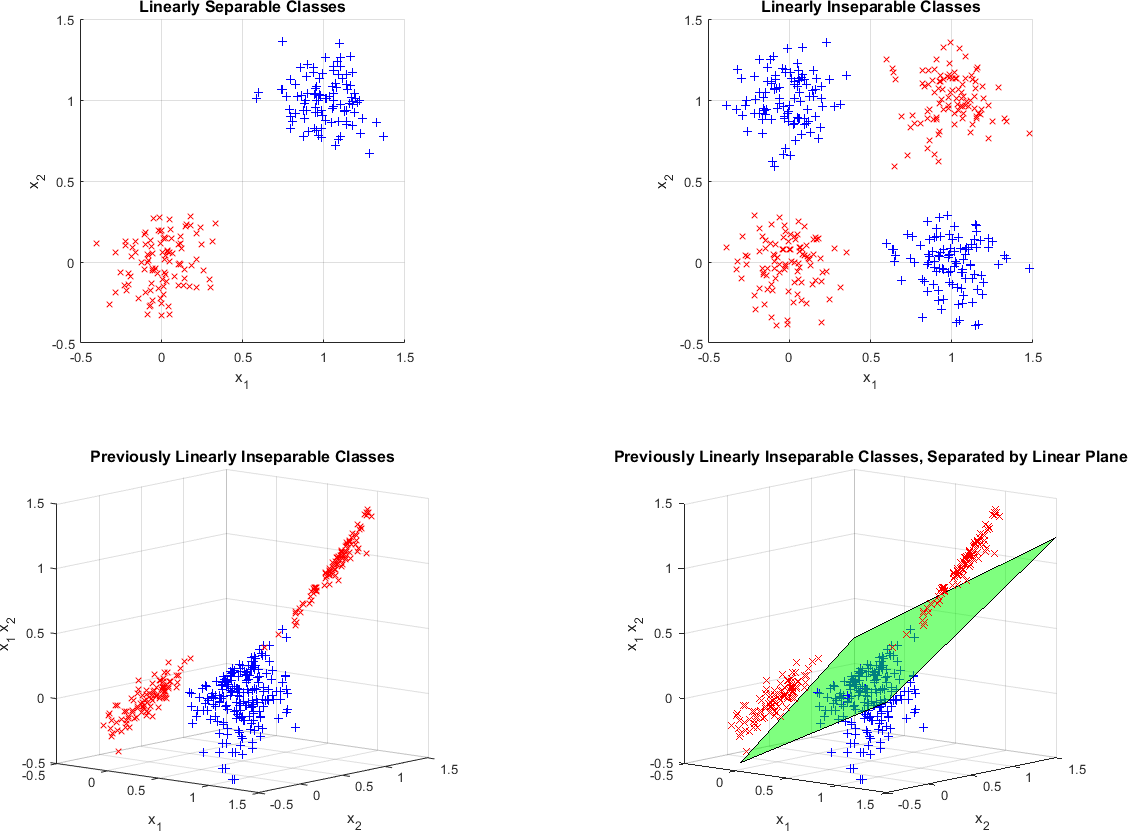
\includegraphics[width=\textwidth]{SVMDataCrop.png}
	\caption[Example of the kernel trick]{Separating linearly inseparable data by introducing an additional dimension\footnotemark}
	\label{fig:SVMSep}
\end{figure}

\footnotetext{The additional dimension is $x_1x_2$. The green plane indicates the plane of separation between classes}

Support Vector Machines (SVMs) are currently the gold standard for learning problems where
the availability of data is not sufficient for a well-trained NN\cite{Fernandez14}. Because sentiment
labelling of the Twitter dataset was performed manually, the SVM is a prime candidate
for our problem of sentiment classification.

SVMs tackle the problem of efficiently computing a model
for linearly inseparable data. \cref{fig:SVMSep} displays the usage of the \textbf{kernel trick}, which is the
introduction of new dimensions dependent on the original dimensions in order to increase linear separability.
This is the main idea behind SVMs.

In order to understand SVMs, we must first delve into pattern recognition theory.
A pattern recognition classifier estimates a function

\begin{align}
\begin{split}
	&f:\R^N \rightarrow \{\pm 1\}\\
	&f(\vec{x}_n) = y_n
\end{split}
\end{align}

where N is the dimensionality of the input vector, and $\vec{x}_n$ and $y_n$ are the input vector and
correct label of the example $n$, respectively\cite{Hearst98}. This function aims to correctly classify
\textit{new} examples -- examples that were not included in the training set but are sampled from
the same distribution. If we put no restrictions on the estimation of $f$, the created function
may perform exceedingly well on the training data, but fail miserably on the unseen data. Such a
classifier would be effectively useless in the real world. Statistical learning theory shows that
we must restrict the class of functions that the machine can learn to one with a suitable \textit{capacity}
for our training data\cite{Vapnik99Stats}. This capacity can be seen as the complexity of the function, in the sense that a highly
complex function (e.g. high-degree polynomial) should not be used to model linearly correlated data.

The discriminator for an SVM is based on hyperplanes
\begin{equation}
	h(\vec{x}) = \vec{wx} + b
\end{equation}

corresponding to the decision function:
\begin{equation}
f(\vec{x}) = \text{sign}(\vec{wx} + b)
\end{equation}

Note that the class labels for a typical SVM are either $-1$ or $1$.
The optimal hyperplane is defined as the hyperplane with the maximum separation
between two classes, such that the Euclidean distances (or margins) between the closest examples of each class
to the hyperplane are maximised. This optimal solution also has the lowest capacity.

In order to make this linear classifier non-linear, we can introduce \textbf{basis functions} $\phi_i$\cite{Holden18}

\begin{align}
\begin{split}
	\vec{\Phi}^T(\vec{x}) &= 
	\begin{bmatrix}
	\phi_1(\vec{x})\ \phi_2(\vec{x}) \dots \phi_k(\vec{x})
	\end{bmatrix}\\
	h(\vec{x}) &= \sigma (\vec{w}^T\vec{\Phi}(\vec{x}) + b)
\end{split}
\end{align}

These basis functions can then be transformed into kernels $K(\vec{x}_i,\vec{x})$:

\begin{align}
\begin{split}
	h(\vec{x}) &= \text{sign}(b + \vec{w}^T\vec{\Phi}(\vec{x}))\\
	&=\text{sign}(b + \sum_{i=1}^m \alpha_iy_i\vec{\Phi}^T(\vec{x}_i)\vec{\Phi}(\vec{x}))\\
	&=\text{sign}(b + \sum_{i=1}^m \alpha_iy_i K(\vec{x}_i,\vec{x}))
\end{split}
\end{align}
where $m$ is the total number of training examples, and $\vec{w} = \sum_{i=1}^m \alpha_iy_i\vec{\Phi}(\vec{x}_i)$
arises from solving
the constrained optimization problem:\\

\noindent Minimise
\begin{equation}
\frac{1}{2}||\vec{w}||^2 + C \sum_{i=1}^m \xi_i
\end{equation}
such that
\begin{equation}
y_if(\vec{x}_i) >= 1-\xi_i\ \text{and\ } \xi_i >= 0\ \text{for\ } i = 1,...,m
\end{equation}
by solving the Lagrangian
\begin{equation}
\begin{split}
L(\vec{w}, b, \vec{\xi}, \vec{\alpha}, \vec{\lambda}) &= \frac{1}{2}||\vec{w}||^2 + C \sum_{i=1}^m \xi_i\\
&\quad - \sum_i\alpha_i(y_if(\vec{x}_i) + \xi_i - 1) - \sum_i\lambda_i\xi_i
\end{split}
\end{equation}
where minimizing $\frac{1}{2}||\vec{w}||^2$ is equivalent to maximizing margins, $\vec{\xi}$ is the measurement
of error(misclassification) and
$C \sum_{i=1}^m \xi_i$ is minimised for minimal error for some hyperparameter $C$\footnote{The exact methods for solving this
optimization problem are beyond the scope of this project and will not be discussed}.

The two most common kernel functions are the Polynomial Function
\begin{equation}
	K_{cd}(\vec{x},\vec{x}') = (c + \vec{x}^T\vec{x}')^d
\end{equation}
where $c$ and $d$ are hyperparameters, and the Radial Basis Function (RBF)
\begin{equation}
	K_{\sigma^2}(\vec{x},\vec{x}') = e^{-\frac{1}{2\sigma^2}||\vec{x}-\vec{x}'||^2}
\end{equation}
where $\sigma$ is a hyperparameter. We will be using the RBF kernel for sentiment classification.

\subsection{Naive Bayes}
\label{sec:introNB}

When tackling a complex learning problem, it is good practice to start by using
a simple model. A Naive Bayes (NB) model is an application of
Bayes' theorem for classification based on conditional probability, 
with the `naive' assumption that the random variables
constituting features are \textbf{independent}. While this assumption isn't completely valid for
most ML problems, it allows us to use an easily built model that often produces
good results regardless of dependent features.

The key idea of NB is to classify an example 
\begin{equation}
\vec{x} = [x_1\ x_2\ ...\ x_n]
\end{equation}
as a class 
\begin{equation}
C_k \in \{C_1, C_2, ..., C_K\}
\end{equation}
by choosing the class $C_k$ representing by
\begin{equation}
\Pr(C_k | x_1\ x_2 ...\ x_n)
\end{equation}
which is the probability
that an example is of class $C_k$ conditioned on its features, which are assumed to be independent
\footnote{Note that $K$ denotes the total number of possible classes}. By application of
Bayes' theorem:
\begin{equation}
\Pr(C_k | \vec{x}) = \frac{\Pr(C_k)\Pr(\vec{x}|C_k)}{\Pr(\vec{x})}
\end{equation}
In practice, we are only concerned with the numerator, since $\Pr(\vec{x})$ is not dependent
on the class $C_k$. $\Pr(C_k)\Pr(\vec{x}|C_k)$ is equivalent to $\Pr(\vec{x}\ C_k)$, and thus:
\begin{align}
\begin{split}
\Pr(\vec{x}\ C_k) &= \Pr(x_1\ x_2\ ...\ x_n\ C_k)\\
&= \Pr(x_1 | x_2\ ...\ x_n\ C_k)\Pr(x_2\ ...\ x_n\ C_k)\\
&= \Pr(x_1 | x_2\ ...\ x_n\ C_k)\Pr(x_2 | x_3\ ...\ x_n\ C_k)\Pr(x_3\ ...\ x_n\ C_k)\\
& \quad\ \vdots\\
&= \Pr(x_1 | x_2\ ...\ x_n\ C_k)\Pr(x_2 | x_3\ ...\ x_n\ C_k)\ ...\ \Pr(x_n\ C_k)\\
&= \Pr(x_1 | x_2\ ...\ x_n\ C_k)\Pr(x_2 | x_3\ ...\ x_n\ C_k)\ ...\ \Pr(x_n | C_k)\Pr(C_k)
\end{split}
\end{align}

Since we made the assumption that each feature is independent

\begin{equation}
\Pr(x_1 | x_2\ ...\ x_n\ C_k)\Pr(x_2 | x_3\ ...\ x_n\ C_k)\ ...\ \Pr(x_n | C_k)\Pr(C_k)
= \Pr(C_k)\prod_{i=1}^n \Pr(x_i | C_k)
\end{equation}

Our classifier's output is then $h = C_k$ for the class satisfying

\begin{equation}
\argmax_k\quad \Pr(C_k)\prod_{i=1}^n \Pr(x_i | C_k)
\end{equation}

The probability $\Pr(C_k)$ can estimated by counting
the number of training examples in each class:
\begin{equation}
\Pr(C_k) \approx \frac{\text{count}(y = C_k)}{\text{count}(y)}
\end{equation}

The types of NB classifiers, such as Gaussian Naive Bayes and Multinomial Naive Bayes,
differ in the assumed distributions of $\Pr(x_i | C_k)$. 

For Gaussian NB, the likelihood of a feature is assumed to be Gaussian:
\begin{equation}
	\Pr(x_i | C_k) \approx \frac{1}{\sqrt{2\pi\sigma_{C_k}^2}} \exp\bigg(-\frac{(x_i - \mu_{C_k})^2}{2\sigma_{C_k}^2}\bigg)
\end{equation}

Similarly, for Multinomial NB, the likelihood of a feature is assumed to be Multinomial. This is used
for when the features are simply counts of distinct events. The 
conditional probability is estimated\cite{Manning08}:
\begin{equation}
	\Pr(x_i | C_k) \approx \frac{1 + \sum_j^n x_i^j}{1 + \sum_m^n \sum_j^n x_m^j} \qquad \forall j.\ y^j=C_k
\end{equation}
where the addition of 1 to both the numerator and denominator is known as Laplace smoothing, or add-one smoothing.
This is to prevent the overall probability for an example belonging to a class being 0 if one or more features had 
never been seen for examples of the class.

A further optimization to combat decimal underflow is to instead calculate the logarithm of this conditional probability,
since $\log$ is a monotonically increasing function and no probability for any class should $= 0$.
\begin{align}
&\argmax_k\quad \Pr(C_k)\prod_{i=1}^n \Pr(x_i | C_k)\\
&=\argmax_k\quad \log\Big(\Pr(C_k)\prod_{i=1}^n \Pr(x_i | C_k)\Big)\\
&= \argmax_k\quad \log\big(\Pr(C_k)\big) + \sum_{i=1}^n \log\big(\Pr(x_i | C_k)\big)
\end{align}

\subsection{Rejected Approach}
\label{sec:prepRej}

As an initial approach to the sentiment analysis problem, \textbf{semi-supervised learning} was attempted
on a large Twitter dataset, as a possible alternative to supervised learning. This meant a much larger dataset
was used, with only a small subset of the data being labelled. The classifier was an iterative application
of an SVM on the labelled dataset, where it would find the unlabelled examples that were clearly
separated by the decision boundary and assign the predicted label to those examples. The training process
was then re-run with the newly autonomously labelled examples in the training set, until all examples
were eventually labelled by the SVM. This process is known as \textbf{Label Spreading}.

\cref{sec:semi} gives an overview of the implementation of this model, and the reasons why it was
ultimately scrapped.

\section{Requirements Analysis}
\label{sec:introReq}
Having studied the basics of Recurrent Neural Networks, Support Vector Machines, and
Naive Bayes, the project requirements were decided. The aim of the project is to
perform sentiment analysis on Twitter news headlines, and use the results as well as financial time-series data
to predict stock market prices with an LSTM. This splits the project into two main logical groups --
the sentiment analysis and the stock price prediction.

\subsection*{Sentiment Analysis}

The most important goal of the Sentiment Analysis part of the project is to
have a high enough accuracy that the output is useful for the stock price
prediction. In terms of functional requirements, several classifiers must be
implemented, and from those I will select the most suitable one for use
with the LSTM. These classifiers will be the Support Vector Machine,
Multinomial Naive Bayes, and Gaussian Naive Bayes. 

Because of the need for Twitter data that matches both the time period and
subject matter of the financial data, I will build a data scraping and processing
system to gather my dataset. I will also be experimenting
with several feature extraction methods from the Twitter dataset, which are
Doc2Vec\cite{Le14} and Bag of Words.


\subsection*{Stock Price Prediction}

The ultimate goal of the project is to be able to predict stock
prices more accurately than a random agent is able to. This accuracy
is a performance measurement of the LSTM model used for predicting
stock prices. The functional requirements for the price prediction
portion of the project are that the sentiment classification output
must combine with the financial data, a feature extractor for financial
indicators must be built, and that the LSTM must function properly, with
well-tuned hyperparameters.

A summary of the requirements for this project is shown in \cref{table:req}.

\begin{table}[H]
\centering
\begin{tabular}{llll}
\toprule
\textbf{Requirement}                                                                               & \textbf{Priority} & \textbf{Risk} & \textbf{Difficulty} \\ \midrule
Multinomial Naive Bayes                                                                                     & Medium            & Medium        & Medium              \\ [0.5ex]
Gaussian Naive Bayes                                                                                        & Medium            & Medium        & Medium              \\ [0.5ex]
Support Vector Machine                                                                                                & High              & Medium        & Low                 \\ [0.5ex]
Twitter data processing                                                                            & High              & Medium        & Medium              \\ [0.5ex]
\begin{tabular}[c]{@{}l@{}}Compare and evaluate Twitter feature \\[-0.5ex] extraction methods\end{tabular} & Low               & Low           & Medium              \\ [2ex]
\begin{tabular}[c]{@{}l@{}}Compare and evaluate sentiment \\[-0.5ex] analysis models\end{tabular}          & High              & Low           & Medium              \\ [2ex]
\begin{tabular}[c]{@{}l@{}}Combine sentiment classifier output\\[-0.5ex] and financial data\end{tabular}   & High              & Medium        & Medium              \\ [2ex]
Feature extractor for financial data                                                               & Medium            & Low           & Medium              \\ [0.5ex]
Long Short-Term Memory Network                                                                                               & High              & High          & High                \\ [0.5ex]
Hyperparameter tuning                                                                              & Medium            & Low           & Medium              \\ [0.5ex] \bottomrule
\end{tabular}
\caption{Goals of the project}
\label{table:req}
\end{table}


\section{Choice of Tools}
\label{sec:introTool}

\subsection{Programming Language}

For machine learning projects, it is quite standard to use \texttt{Python},
because of its support for useful ML libraries (such as Tensorflow, Keras, Theano), its
ease of use and readability, and relaxed type system. Though the language is not as
fast as other languages such as \texttt{Java} and \texttt{C++}, many of its
powerful libraries use \texttt{CPython}, which is a reference implementation
and interpreter of \texttt{Python} in \texttt{C}.
This allows these libraries to exploit the performance of \texttt{C} while maintaining
the benefits of \texttt{Python}. I have chosen to use \texttt{Python} as the main
language for my project, while also using \texttt{MATLAB} for some trivial
plotting and mathematical tasks.

\subsection{Libraries}
\label{sec:introLib}

The main third party libraries used are shown in \cref{table:libs}. Tensorflow\footnote{https://www.tensorflow.org/}
and Scikit-learn\footnote{http://scikit-learn.org/} are
of particular importance. Both libraries are well-documented and widely used in industry, with the 
latter often being used for prototyping. GetOldTweets\footnote{https://github.com/Jefferson-Henrique/GetOldTweets-python}
is not an official library, but is an open-source
project for scraping Twitter searches to retrieve Tweets that are older than allowed by the official Twitter 
API's query limit.

\begin{table}[H]
\centering
\begin{tabular}{llll}
\toprule
\textbf{Library}                        & \textbf{Version} & \textbf{Use} & \textbf{License} \\ \midrule
Tensorflow                             & 1.5.0            & Building LSTM        & Apache 2.0 License              \\ [0.5ex]
Scikit-learn                           & 0.19.0           & Using SVM        & BSD-new License              \\ [0.5ex]
Numpy                                  & 1.14.0           & Efficient array manipulation        & BSD-new License              \\ [0.5ex]
Scipy                                  & 0.19.1           & Probability functions for NB        & BSD-new License              \\ [0.5ex]
Pandas                                 & 0.20.3           & Data manipulation        & BSD-new License              \\ [0.5ex]
Gensim								   & 2.3.0			  &	\texttt{Doc2vec} feature extraction			& GNU LGPLv2.1 license\\ [0.5ex]
Matplotlib							   & 2.0.2			  & Graph plotting 				& Matplotlib License	\\ [0.5ex]
GetOldTweets                           & Unknown          & Twitter web scraping        & MIT License              \\ [0.5ex] \bottomrule
\end{tabular}
\caption{Main libraries used in this project}
\label{table:libs}
\end{table}

\subsection{Development and Testing}

Development was carried out on my personal laptop, which runs Windows 10. Because of its relatively 
powerful graphics card (Nvidia GTX 1060), it was also capable of training and testing the LSTM
models.

For revision control, I used \texttt{git}, the revision control system
that is almost ubiquitous in industry. I created and synchronised repositories on
GitHub\footnote{https://github.com, a free and popular \texttt{git} repository hosting service}, 
for both my project and the dissertation write-up. This was used not only for
planning and tracking progress, but also as a back-up tool. 


\section{Starting Point}
\label{sec:introStart}

The Computer Science Tripos has several courses that proved useful for my project.
These are outlined in \cref{table:courses}. In particular, Machine Learning and
Bayesian Inference provided me with the base knowledge required for understanding
SVMs, Naive Bayes, and Neural Networks -- however, personal study was required to
learn about RNNs and LSTMs, as well as different hyperparameter tuning techniques.

My knowledge of \texttt{Python} prior to this project was intermediate, having used it
only as a minor part of a prior internship. I had no experience with Tensorflow
or other Deep Learning libraries. This meant I had to learn the design concepts
behind Tensorflow, which is to construct mathematical operations for NNs as
computational graphs operating on tensors. 

\begin{table}[H]
\centering
\begin{tabular}{llll}
\toprule
\textbf{Course}                              & \textbf{Application} \\ \midrule
Machine Learning and Bayesian Inference      &  Neural Networks, SVM                    \\
Natural Language Processing                  &  Twitter feature extraction                    \\
LaTeX and MATLAB                             &  Plotting       \\
Mathematical Methods for CS    &  Understanding probability functions            \\
Software Engineering                         &  Iterative development model                    \\\bottomrule
\end{tabular}
\caption{Tripos courses applicable to this project}
\label{table:courses}
\end{table}

\section{Software Engineering and Approach}
\label{sec:introImpl}

For a project of this scale, it is imperative to plan the different stages of
development, and to compartmentalise the project. As was already outlined in \cref{sec:introReq},
the project was split into two main sections: sentiment analysis and stock price prediction. An
overview schematic of the project's components are show in \cref{fig:overview}.

\begin{figure}[H]
\centering
\vspace{10pt}
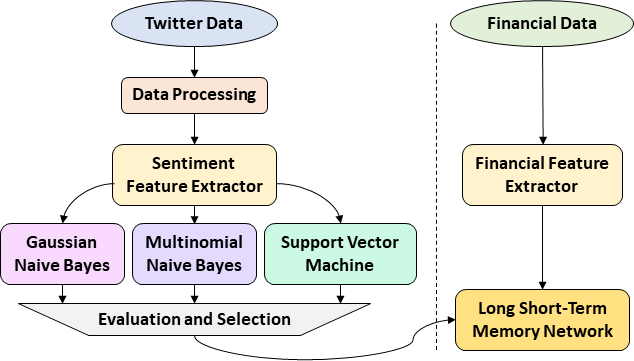
\includegraphics[width=\textwidth]{Proj_Overview.png}
\caption{Overview of project components}
\label{fig:overview}
\end{figure}

The \textbf{Iterative and Incremental Development Model} was adopted for this project.
The idea was to first build a `walking skeleton', an runnable end-to-end system that
has all of the essential components of the final end-product, though the components
may simply be placeholders\cite{Cockburn04}. These components can then be properly
implemented at a later date, with the project's architecture already in place.
These components were then iteratively tuned and improved.

The list of components to complete were as follows, ranked by implementation order:

\begin{enumerate}
\item
Collect Twitter and financial data

\item
Build Twitter data processing system

\item
Manually label Twitter dataset

\item
Implement sentiment feature extractors

\item
Build Gaussian and Multinomial Naive Bayes

\item
Build SVM

\item
Evaluate and pick the best-performing classifier

\item
Implement financial feature extractor

\item
Build LSTM
\end{enumerate}
The components described in steps 4-9 were then iteratively refined after initial completion.


\section{Summary}
\label{sec:prepSumm}

In this chapter, I have discussed the relevant theory that had to be understood, the planning
that occurred, before implementation was started. I gave an introduction to the concepts
behind the machine learning models I will be implementing, and outlined the goals and
key development strategies. I have also given an overview of the tools and libraries I
will be using.

The next chapter will detail the implementation of the project, showing how the goals and
plans outlined in this chapter were achieved.

\chapter{Implementation}
\label{sec:imp}

This chapter details the implementation of the project, and how the goals and
design principles outlined in the previous chapter were accomplished. I will be
presenting the sentiment analysis portion of the project first, before moving into price
prediction section. This was the order in which I implemented the project, as outlined
in the previous chapter, and provides a logical flow between the components.

\todo[inline]{TODO: find a place to fit this: Multinomial Naive Bayes, Gaussian Naive Bayes, and Multi Class
Support Vector Machines, using different methods of feature extraction, were used to classify the
sentiment of relevant Twitter posts of news headlines. The Long Short-Term Memory (LSTM) Recurrent 
Neural Network (RNN) was used for predicting stock prices, utilizing both
financial technical indicators and the output of the sentiment classifiers.}

\section{Sentiment Analysis}
\label{sec:impSenti}
This section first gives an overview of the initial rejected approaches to the
learning problem. The rest of the section is discussed in the logical order of data flowing 
through the system --
we discuss the collection of data, before
moving onto feature extraction, and finally the different sentiment classifiers.

\subsection{Rejected Approach}
\label{sec:impFailed}

This section details the initial approach to the sentiment analysis problem
that was ultimately scrapped.

\subsubsection{Semi-Supervised Learning}
\label{sec:semi}
My first experimental forays into the sentiment analysis problem was to
simply acquire as much relevant data as I could, and manually label a small subset
to feed into a semi-supervised learning model. The initial reasons behind this decision
were that there was a large abundance of official Twitter accounts of large news
agencies, and that there may be a sufficiently large number of samples for a
semi-supervised Deep Learning model, such as a \textbf{Hybrid Deep Belief Network}\cite{Zhou14}.

My approach to examining potential solutions to a learning problem is to first
use a simple model in order to gain insight on whether the problem can feasibly
be solved. Following this ethos, I used Scikit-Learn's semi-supervised learning module's
label spreading implementation to test the feasibility of using a semi-supervised learning
method for this dataset. This module uses the label spreading method mentioned in
\cref{sec:prepRej}, combined with a standard SVM.
After manually labelling around 2000 tweets, out of
approximately 500,000 tweets, I separated the labelled dataset into an 80:20 split for train:test,
a standard ratio for partitioning data. The labelled 80\% training set was then combined
with the rest of the unlabelled dataset and used to train the semi-supervised SVM. The
trained model was then evaluated on the separated labelled test dataset. 

The results gave very little confidence in moving forward with this technique, as the accuracy 
for sentiment classification was 54%. Considering the output of the sentiment classifier is
to be fed into the LSTM network as an input, it was imperative that the output be mostly correct,
in order to ensure that inputs to the LSTM are kept as noise-free as possible. Thus, I decided to
pursue a supervised learning approach to the sentiment analysis problem.

\subsection{Data}
\label{sec:impSentiData}

After experimenting with semi-supervised learning, I quickly realized
that it may be more effective to be selective about the data I was collecting. This ensures
that I have a dataset that was small enough to manually label and further enforces that only relevant 
information to the price prediction model should be used. 

I settled on using tweets from the official Reuters Twitter account\footnote{\url{https://twitter.com/Reuters}}.
From reading through the semi-supervised dataset, I quickly realized that there was a great deal of redundancy
when sampling from many news agencies, as any important news story is often broadcasted by most agencies.
I chose Reuters because it is a leading provider of financial news, and
most news regarding specific companies that were registered on the stock exchange of
study, NASDAQ, were labelled with the corresponding ticker symbol\footnote{A ticker symbol is the identifier given to a company on
a stock exchange}. In order to account for irregularities in tweet styles,
I also performed a search for mentions of the company's name in each tweet. This also 

\subsubsection{Initial Approaches}
My first approach to acquiring the Twitter dataset was to try to find labelled datasets from other studies
that have been conducted regarding Twitter sentiment analysis on financial data. After failing to find any that 
were sufficiently related to the aims of my project, I moved to collect the data through Twitter's official web API.
However, after discovering that the API calls for retrieving tweets that are older than a week were locked
behind various paywalls\footnote{\url{https://developer.twitter.com/en/docs/tweets/search/overview}}, I decided to find a way around this issue.

\subsubsection{Crawling}
\label{sec:impCrawl}

As was mentioned in \cref{sec:introLib}, I used the GetOldTweets library for web scraping the relevant Twitter page.
The aforementioned limitation on historical tweet retrieval prevented me from acquiring data that matched the 
full time period of my financial data, as my financial dataset required a sufficiently large number of samples 
for a Deep Learning model.

This library generates a search query URL on Twitter, which specifies the username, time frame, language,
search query, and maximum number of returned tweets. An HTTP GET request is then sent to the search URL,
and the JSON-formatted response of the search results in returned. This response only contains a page
worth of results, so the process is repeated until all results are gathered. This response is then parsed and
converted to a custom Tweet object, and returned from the original function call.

\subsubsection{Labelling}
\label{sec:impLabel}
\todo[inline]{TODO: This section, discuss criteria for labelling pos/neg}

\subsubsection{Pipeline}
\label{sec:impPipeline}

\todo[inline]{TODO: MAYBE SCRAP THIS SECTION}

The pipelining process was designed around disk I/O. This means that when data travels through the pipeline,
it is written to file at each stage, in order to ease debugging and increase transparency, but also to
preempt scalability issues in future applications of the pipeline where the data may not fit entirely in memory.
This is often the case for machine learning problems in industry, where dataset files can span terabytes
\footnote{An example of a standard dataset of this size is the Google Books Ngrams dataset, which is 2.2 TB. 
\url{https://aws.amazon.com/datasets/google-books-ngrams/}}.

Another reason for basing the pipeline around file I/O is that this dataset required manual labelling.
This means there is a specific stage of the pipeline where the user must open the required temporary
file and manually comb through the Twitter data, before the next function can be run and the file
be converted to the requisite datatype.

The pipeline's goals between its stages are to:

\subsection{Features}
\label{sec:impSentiFeat}
There are three main feature extraction systems that I used for the Twitter dataset. The first is
a simple Bag of Words approach. This is the vector representation for word occurrence counts --
we first build a vocabulary of words by parsing through the training dataset to find a list of all unique words,
and assigning an index to each unique word. We then build feature vectors of $m$ length, where $m$ is the
total number of unique words in the dataset. Then, for every word in the training example, we simply
increment the value at the corresponding index for the word in the feature vector. This can intuitively
be explained as a tally for each unique word in the example, with zeros in the dimensions where the
corresponding word does not appear in the example. 

\missingfigure[figheight=6cm]{TODO: BOW FIGURE}

For cases where unique words may appear in the test/validation
dataset that did not appear in the training set, we can either initially include an extra dimension in the feature
vector for `other', but in the case of our models, since the training data does not include any examples featuring
this word, the model will either not have trained to include it in its decision boundary, or unexpected
behaviour may occur. Thus, it is better practice to simply omit new unique words when extracting features
from the test/validation sets.

The current state-of-the-art feature representation method for text is \texttt{doc2vec}\cite{Le14}.
This method is a continuation of \texttt{word2vec}\cite{Mikolov13}. \texttt{Word2vec} is a method
for vector representation of a word generated through unsupervised learning. The idea of this method
is that words of similar semantic meaning are closer by Euclidian distance in the feature vector space than
words that are not semantically related. \cref{fig:word2vec} shows this property. It also shows that logical vector relations 
also follow from this property, in the sense that the feature vector for a word can be deconstructed as the
combination of two or more feature vectors that are logically computed in the realm of semantic relations.
The example shown in the figure is that $\vec{King}$ is to $\vec{Queen}$ what $\vec{Man}$ is to $\vec{Woman}$,
and $\vec{King} - \vec{Man} + \vec{Woman} = \vec{Queen}$. This shows that
logical combinations of words' semantic meanings are directly translated to addition and subtraction in
the feature vector space.

\begin{figure}[H]
\centering
\vspace{10pt}
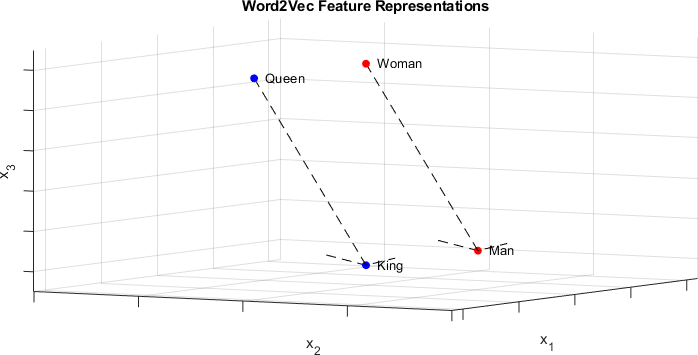
\includegraphics[width=\textwidth]{word2vec.png}
\caption{Simplified \texttt{word2vec} representation of words}
\label{fig:word2vec}
\end{figure}

This feature representation is generated through an unsupervised feedforward neural network. There
are two models for \texttt{word2vec} -- \textbf{continuous bag of words} (CBOW) and \textbf{skip-gram}.
CBOW is a bag of words method that takes into
account the context of a word and tries to predict this word whose context it has been given.
CBOW takes the one-hot-encoding vectors
for words within a given window around the selected word in a sentence. These vectors are averaged,
and fed through a feedforward neural network with a single hidden layer 
and output layer to try to predict the selected word. The output layer is what's known as a \textbf{softmax}
layer, which is a generalized version of the logistic sigmoid function explained in \cref{sec:prepNeurons},
applying the sigmoid function to every element of a vector.
The weights for this hidden layer, after training, are then translated into the feature extractor.
The skip-gram model works in the opposite
direction -- given a selected word, it predicts the
context of the word (average of the words within the specified window around the selected word).
The skip-gram model is much slower to train, but is more accurate for infrequent words.
Due to the repetitive nature of our dataset, we will be using CBOW.

\missingfigure[figheight=6cm]{TODO: FIGURES OF WORD2VEC}

The \texttt{doc2vec} method abstracts the \texttt{word2vec} methods to a vector representation
for a whole document. The model predicts the a word within a paragraph given its context, as well
as a paragraph ID, represented in a one-hot-encoding vector. The context and paragraph ID can then
be either averaged together, such as in CBOW in \texttt{word2vec}, or concatenated. Averaging
results in a model that disregards word order, but requires substantially fewer
examples to train. We will be using the averaging method, as our dataset is not sufficiently
large for concatenation. The architecture for single hidden layer and softmax output layer are
the same as for the \texttt{word2vec} model, meaning we use the hidden layer's weights as our
feature extractor after training the \texttt{doc2vec} model.

\missingfigure[figheight=6cm]{TODO: FIGURES OF DOC2VEC}

\subsection{Naive Bayes}
\label{sec:impNB}
This section will explain the implementation of each Naive Bayes classifier.

The following two versions of the Naive Bayes classifier were chosen because they are seemingly
well-suited to our two feature extraction methods. Gaussian Naive Bayes, which accepts an input
feature vector of real values (with the assumption that the features have a Gaussian distribution),
is the most fitting NB classifier for \texttt{doc2vec}. Multinomial Naive Bayes,
which accepts an input feature vector where each feature is a count of an event (with the assumption
that the counts have a Multinomial distribution), is perfect for Bag of Words.

\subsubsection{Gaussian Naive Bayes}
\label{sec:impGNB}

Gaussian Naive Bayes was implemented by

\subsubsection{Multinomial Naive Bayes}
\label{sec:impMNB}




\subsection{Support Vector Machine}
\label{sec:impSVM}

\section{Price Prediction}
\label{sec:impFin}
This section will detail the implementation of the price prediction portion
of the project. We will discuss the decisions behind data selection,
the different technical features that were chosen, and the implementation
of the LSTM network.

\subsection{Data}
\label{sec:impFinData}

Because of the need for manual labelling of the Twitter dataset, as mentioned in \cref{sec:impFailed} and 
\cref{sec:impSentiData}, a financial dataset with specific requirements was chosen:

\begin{itemize}
\item
The dataset must not span too large a time period, to ensure the corresponding Twitter dataset is not too large to label

\item
The dataset must not include too many stocks, to ensure the corresponding Twitter dataset is not too large to label

\item
The dataset must include enough samples, to ensure the LSTM network has sufficient data for training

\item
The dataset must be composed of relevant stocks whose companies regularly receive media attention

\item
The dataset preferably includes a representative group of stocks for an industry or the global economy

\end{itemize}

The resulting dataset comprises of a 6-month period of data for the five highest market cap\footnote{Market cap, 
or market capitalization, is the total market value of a company's shares} stocks on the
NASDAQ exchange: Apple, Amazon, Alphabet\footnotemark ($\times2$), and Microsoft.


\footnotetext{Alphabet is listed twice on the NASDAQ exchange, as GOOGL and GOOG. These are two separate stocks: GOOGL
holders have voting rights while GOOG holders do not}

\subsection{Features}
\label{sec:impFinFeat}

\todo[inline]{Write about technical indicators}

\begin{table}[H]
\centering
\begin{tabular}{ll}
\toprule
\textbf{Feature}          					& \textbf{Description} \\ \midrule
\begin{tabular}[c]{@{}l@{}}Williams percentage range\\(Williams \%R)\end{tabular}	& \begin{tabular}[c]{@{}l@{}}Measures overbought and oversold levels,used\\with an interval to find highest and lowest prices\\during time frame\end{tabular} \\[2.5ex]\midrule
Rate of change (RoC)						& Ratio of change from previous price \\[0.5ex]\midrule
Momentum									& Change of price within an interval \\[0.5ex]\midrule
Relative strength index (RSI)				& \begin{tabular}[c]{@{}l@{}}Compares magnitude of recent gains andlosses\\to measure speed and change ofprice\\movements, primarily used to gauge overbuying\\and overselling\end{tabular} \\[3.5ex]\midrule
\begin{tabular}[c]{@{}l@{}}Triple exponential moving\\average (TEMA)\end{tabular} 	& Smooth price fluctuations and filter out volatility \\[2ex] \bottomrule

\end{tabular}
\caption{Financial technical indicators used as features}
\label{table:fintech}
\end{table}



\begin{itemize}
\item
Williams \%R
\begin{equation}
\frac{\text{highest price} - \text{current price}}{\text{highest price} - \text{lowest price}}
\end{equation}

\item
RoC
\begin{equation}
\frac{\text{current price}}{\text{previous price}} - 1
\end{equation}

\item
Momentum
\begin{equation}
\text{current price} - \text{price at previous interval}
\end{equation}

\item
RSI
\begin{align}
\begin{split}
&\frac{100 \times \text{average}(\text{upgain})}{\text{average}(\text{upgain}) + \text{average}(\text{downloss})}\\
\intertext{where}
\text{upgain} = &\text{price} - \text{previous price} \quad \text{when} \quad \text{price} > \text{previous price}\\
\intertext{and}
\text{downloss} = &\text{previous price} - \text{price} \quad \text{when} \quad \text{price} < \text{previous price}
\end{split}
\end{align}

\item
TEMA


\end{itemize}

\subsection{Long Short-Term Memory}
\label{sec:ImplLSTM}

This section will detail

\todo[inline]{TODO: talk about how not having tweets for a certain time period is fine, because of LSTM architecture}
\todo[inline]{TODO: measure mean and stdev of random agents}

\subsubsection{Initialisation}

\subsubsection{Normalisation}

\subsubsection{Hyperparameters}

\subsubsection{Dropout}

\subsubsection{Early Stopping}



\section{Testing Framework}

\missingfigure[figheight=6cm]{UML diagram of framework}

\subsection{Hyperparameter}

\subsection{Random Agents}


\chapter{Evaluation}

\section{Overall Results}

\section{Hyperparameters}

\section{Testing}

\section{Sentiment Evaluation}

\section{Prediction Evaluation}

\section{Summary}

\chapter{Conclusion}

\section{Results}

\section{Lessons Learned}

\todo[inline]{TODO: mention careful selection of data. would have been better to pick one/two stocks and do daily intervals, so more news for each interval
without overwhelming twitter labelling}

\section{Further Work}

 
%%%%%%%%%%%%%%%%%%%%%%%%%%%%%%%%%%%%%%%%%%%%%%%%%%%%%%%%%%%%%%%%%%%%%
% the bibliography
\addcontentsline{toc}{chapter}{Bibliography}
\bibliography{refs}


%%%%%%%%%%%%%%%%%%%%%%%%%%%%%%%%%%%%%%%%%%%%%%%%%%%%%%%%%%%%%%%%%%%%%
% the appendices
\appendix

\chapter{Latex source}


\chapter{Project Proposal}

\end{document}